
\section{ Постановка задачи }\label{sec:taskdef}

\begin{definition}{\textit{Оптическое распознавание символов (Optical Character Recognition, OCR)}} -- процесс считывания текста с физического носителя и его сохранения в цифровом формате. Текст состоит из \textit{символов}.
\end{definition}

\begin{definition}{\textit{Ошибка OCR}} -- случай, когда очередной символ текста распознался неверно или не распознался. Ведёт к понижению качества распознавания.
\end{definition}

\begin{definition}{\textit{$N$-грамма}} -- последовательность из $n$ элементов (слов, звуков, символов). Анализируя их частотности, можно строить модели для анализа и синтеза языка.
\end{definition}

\begin{definition}{\textit{$N$-граммная модель}} -- вероятностная модель языка, которая рассчитывает вероятность последнего элемента $n$-граммы, если известны все предыдущие. \\
При использовании $n$-граммных моделей предполагается, что появление каждого элемента зависит только от предыдущих элементов.
\end{definition}

\textbf{Цель работы} -- сравнить эффективность различных символьных $n$-граммных моделей в задаче исправления ошибок OCR в японском языке.

Из цели работы вытекают следующие \textbf{задачи}:
\begin{itemize}
	\item Рассмотреть существующие подходы к $n$-граммному моделированию японского языка;
	
	\item Реализовать некоторые модели;
	
	\item Развернуть систему для тестирования и сравнения моделей.
\end{itemize}

Чтобы понять специфику цели работы, нужно учесть особенности японского языка.

Очевидно, что устройство японского языка на уровне конкретных символов сложнее, чем устройство языков латино-романской группы (в которых существует всего 25-40 символов, учитывая возможную диакритику).

\subsection{ Обзор японского языка }

Письменный японский текст -- это комбинация слогово-фонетических символов (кана) и иероглифов (кандзи).
Слоговая азбука кана делится на катакану и хирагану, которые представляют собой разные графические формы одних и тех же слогов. \todo{сказать, почему забиваем на окуригану и т.д.}

Рассмотрим эти символы подробнее:

\begin{itemize}
	\item Хирагана (см. Рис. \ref{fig:hirag_sample}), символы более округлые, чем в катакане. В основном используется для образования грамматических морфем.
	\begin{figure}[H]
		\centering
		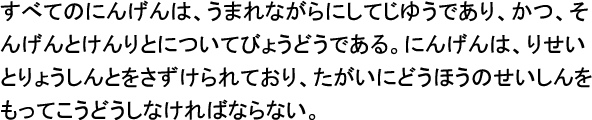
\includegraphics{hirag_sample.png}
		\caption{hirag\_sample}
		\label{fig:hirag_sample}
	\end{figure}
	
	\item Хирагана (см. Рис. \ref{fig:katak_sample}), символы более резкие, чем в хирагане. Используется для транскрибирования иностранных заимствованных слов \todo{примеры :)}.
	\begin{figure}[H]
		\centering
		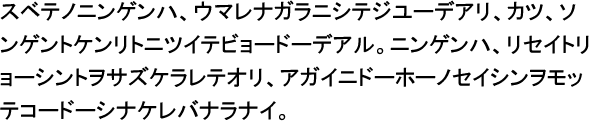
\includegraphics{katak_sample.png}
		\caption{katak\_sample}
		\label{fig:katak_sample}
	\end{figure}

	\item Также есть диакритические символы -- дакутен, хандакутен (\todo{?}) (см. Рис. \ref{fig:dakut_sample}). Они могут применяться как к катакане, так и к хирагане, и определённым образом влияют на звучание слогов.
	\begin{figure}[H]
		\centering
		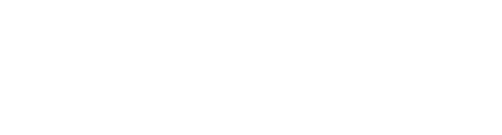
\includegraphics{draft.png}
		\caption{dakut\_sample}
		\label{fig:dakut_sample}
	\end{figure}

	\item Кандзи (см. Рис. \ref{fig:kandji_sample}). Это символы, несущие семантическую нагрузку. С точки зрения написания иероглифы можно поделить на пиктограммы, идеограммы и фонограммы \todo{?}. 
	\begin{figure}[H]
		\centering
		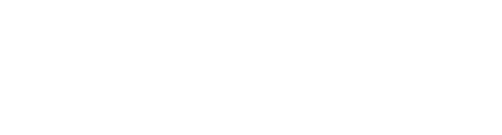
\includegraphics{draft.png}
		\caption{kandji\_sample}
		\label{fig:kandji_sample}
	\end{figure}
\end{itemize}

Кана различает 46 слогов, которые могут записываться как катаканой, так и хираганой. А вот иероглифов кандзи существует гораздо больше (6000 достаточно для жизни, а стандарт Unicode определяет 21000) \todo{цифры}.

Японский текст записывается с помощью комбинаций кандзи, кан и пунктуации, при этом отсутствует пробельное деление предложений на слова (см. Рис. \ref{fig:japtext_sample}).
	\begin{figure}[H]
	\centering
	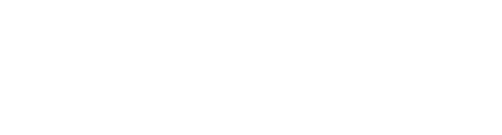
\includegraphics{draft.png}
	\caption{japtext}
	\label{fig:japtext_sample}
\end{figure}

По сравнению с латино-романскими языками, где алфавит меньше в сотни раз, а деление текста на слова очевидно, задача корректного распознавания символов становится значительно сложнее. Это требует более изощрённых подходов для автоматического анализа распознанного текста и поиска ошибок в нём.

Рассмотрим несколько примеров символов, которые легко спутать.

\subsection{ Путающиеся символы в японском }

\begin{itemize}
	\item[2Kana] 2 похожие каны. Таким случаев достаточно мало, а методы их различения уже существуют.
	\begin{figure}[H]
		\center{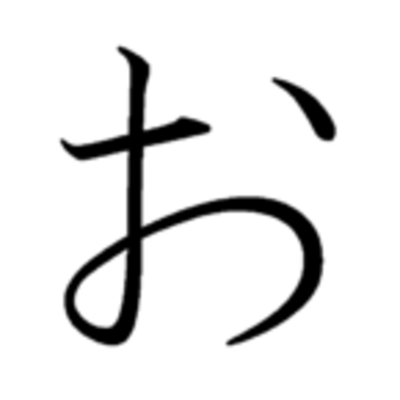
\includegraphics[scale=1.0]{KanaO.png}\ и 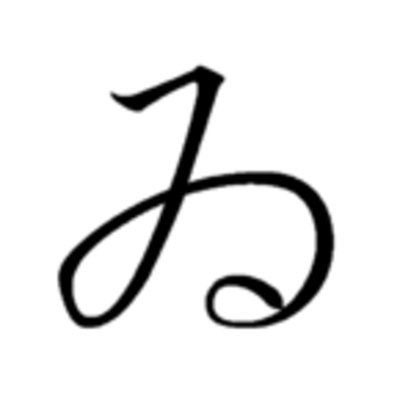
\includegraphics[scale=1.0]{KanaWi.png}}
	\end{figure}

	\item[KaGa] Кана может легко путаться с соответствующим её дакутен-символом.
	\begin{figure}[H]
		\center{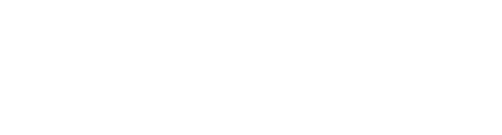
\includegraphics[scale=1.0]{draft.png}\ и 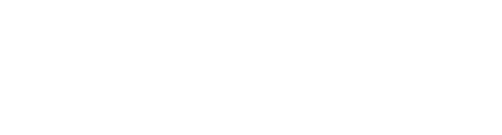
\includegraphics[scale=1.0]{draft.png}}
	\end{figure}

	\item[BigSmall] Существуют большие и маленькие каны, которые нужно различать.
	\begin{figure}[H]
		\center{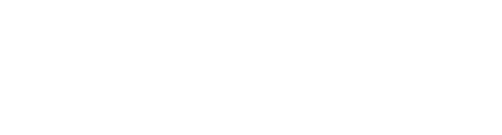
\includegraphics[scale=1.0]{draft.png}\ и 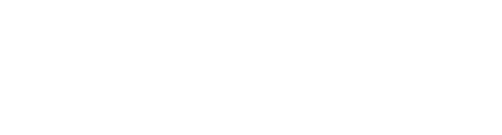
\includegraphics[scale=1.0]{draft.png}}
	\end{figure}

	\todo{HalfWidth?}
	
\end{itemize}

\subsection{ Формальная постановка задачи }

\begin{definition}
	{\textit{Алфавит $\Sigma = \{ a, b, c, .. \}$}} -- множество символов в данном языке. В японском языке их около 80000, стандарт Unicode поддерживает примерно 21000.
\end{definition}

\begin{definition}
	{\textit{Текст $Text \in \Sigma^+$}} -- последовательность символов из алфавита $\Sigma$ положительной длины.
\end{definition}

\begin{definition}
	Текст делится на конечное множество {\textit{предложений $S = \{ S_1, S_2, S_3, ... \}$}} знаками пунктуации и форматированием. $Text = S_1S_2S_3...$.
\end{definition}

Для каждого из предложения текста существует единственно верный вариант написания \todo{а что делаем с омонимией?}, а также некоторое (фиксированное) число неверных. Требуется ответить, какой из вариантов верен.

\begin{definition}
	{\textit{Оценивающий алгоритм (estimator) $\Theta : S \rightarrow \mathbb{R}^+ $}} -- функция, возвращающая оценку правильности варианта $S$.
\end{definition}

Среди $k$ вариантов предложения выбирается наилучший: $S_{best} = \argmaxl_{S} \Theta(S)$, который и считается правильным.

Если $S_{best}$ угадано верно, то на данном предложении алгоритм $\Theta$ отработал правильно.

\begin{definition}
	{\textit{Качество алгоритма $Q(\Theta) = \dfrac{\#\{ \text{угаданных предложений} \}}{\#\{ \text{всего предложений} \}}$}}.
\end{definition}

Задача -- реализовать ряд оценивающих алгоритмов (см. раздел \ref{sec:models}), основанных на $n$-граммных моделях, и сравнить их по качеству.